\section{Evaluation}
\subsection{Storage systems latency.}
We use FIO to measure how much latency each different storage system adds.
Figure \ref{fig:fio_512} shows the latency with \SI{512}{B} request size
of each storage system.

\begin{figure}[H]
  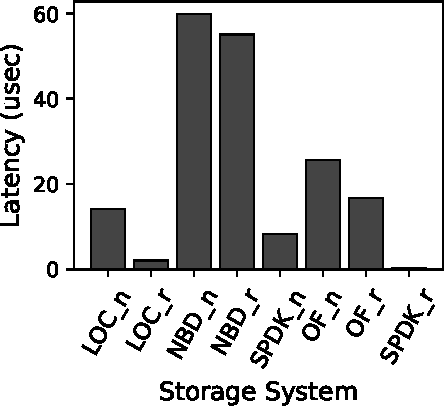
\includegraphics[width=\linewidth]{figures/fio_512.pdf}\\
\caption{Average latency (usec) of local and remote storage systems with \SI{512}{B} request size. "r" stands for ramdisk and "n" stands for NVMe, "OF" stands for NVMe-oF with SPDK User-Space drivers.}
\label{fig:fio_512}
\end{figure}

We will analyze the results to determine the best setup for evaluating TeraHeap. Starting with local SSD FIO reports an average of 14.16 $\mu$s latency and for local ramdisk, FIO reports 2.04 $\mu$s 6.94$\times$ better. First, we will investigate the remote option NBD (TCP). The exported SSD with NBD average latency is 4.22$\times$ higher than local with an average of 59.86 $\mu$s. Meaning that we get 45.7 $\mu$s more latency with NBD. By looking at the exported ramdisk with NBD average latency is 1.08$\times$ better than the NBD SSD, meaning that there is a common overhead. This overhead can either be the NBD I/O path or high TCP latency. We use Netperf ~\cite{netperf} to measure the TCP latency and conduct experiments with \SI{512}{B} of data in each packet. Netperf reports 37.84 $\mu$s average
latency. Adding local NVMe and TCP latency we have 52 $\mu$s 7.86 $\mu$s difference to the NBD
(TCP) latency 59.86 $\mu$s. We conclude that the primary overhead is TCP, accounting for 63.2\% of the average latency in NBD NVMe.

Next, we investigate lowering the latency of the local I/O path to the device by using userspace drivers (SPDK). With userspace drivers, we bypass the layers of the kernel's I/O stack and eliminate context switches ~\cite{spdk}. We run FIO on the NVMe with SPDK and get 8.31 $\mu$s average latency 1.7$\times$ better compared to traditional drivers. We also try to lower
the network latency with NVMe-oF NVMe with SPDK User-Space drivers. With the combination of SPDK’s user-space optimizations, the efficient protocol design of NVMe-oF compared to TCP and RDMA with Infiniband transport layer we manage to measure 25.69 $\mu$s average latency 2.33$\times$ better than SSD with NBD. 

Moving on SPDK ramdisk outperforms everything with 0.33 $\mu$s average latency,
but the NVMe-oF ramdisk with SPDK User-Space drivers have 16.66 $\mu$s average
latency 9.03 $\mu$s better than the NVMe-oF NVMe and only 1.54$\times$ better
compared to the local performance where the local ramdisk is 25.18$\times$
better. There is a common overhead in both NVMe-oF setups which is attributed
either to the NVMe I/O path or network latency. Previously we measured the NVMe
with SPDK User-Space drivers and got 8.31 $\mu$s a logical 32.34\% of the
NVMe-oF NVMe with SPDK latency. We used ib\_read\_lat ~\cite{perftest} to
conduct RDMA Read Latency Test with \SI{512}{B} requests and we measure that the
Infiniband ports average latency is 2 $\mu$s only 7.78\% of the NVMe-oF NVMe
with SPDK latency meaning that the high latency can be by the Linux Kernel
NVMe-oF Initiator which uses traditional kernel I/O calls to the exported device
and then the calls are encapsulated and transported to the target via
Infiniband. Unfortunately, SPDK's user-space NVMe-oF initiator ~\cite{spdk}
doesn't directly create block devices in /dev, SPDK uses its own block
device layer (bdev) which will not be compatible for later experiments with TeraHeap. 

\begin{figure}[H]
  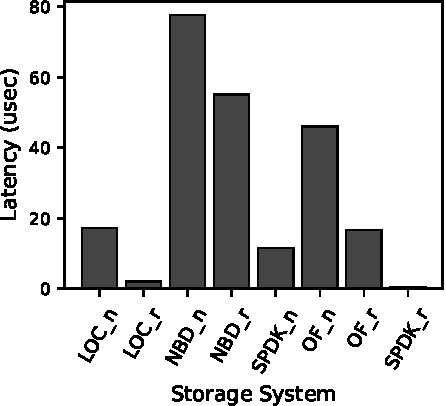
\includegraphics[width=\linewidth]{figures/fio_4k.pdf}\\
\caption{Average latency (usec) of local and remote storage systems with \SI{4}{KB} request size."r" stands for ramdisk and "n" stands for NVMe, "OF" stands for NVMe-oF with SPDK User-Space drivers.}
\label{fig:fio_4k}
\end{figure}

Similarly, with \SI{4}{KB} block size we get the same overheads as shown in figure
\ref{fig:fio_4k}. Here FIO reports more latency for moving the \SI{4}{KB} data locally
and/or across network. The NVMe-oF NVMe with SPDK achieving 25.69 $\mu$s and the
NVMe-oF ramdisk with SPDK reaching 16.66 $\mu$s average latency (nearly as fast
as the local NVMe at 14.16 microseconds) are suitable to proceed with our
evaluation using TeraHeap.



\subsection{TeraHeap performance with NVMe-oF}
\par This section compares TeraHeap performance of two setups one with local NVMe device and one with NVMe-oF exported NVMe with SPDK User-Space drivers. Figure \ref{fig:bench_spark} illustrates the performance of TeraHeap with Spark workloads for both setups. 
\begin{figure}[H]
  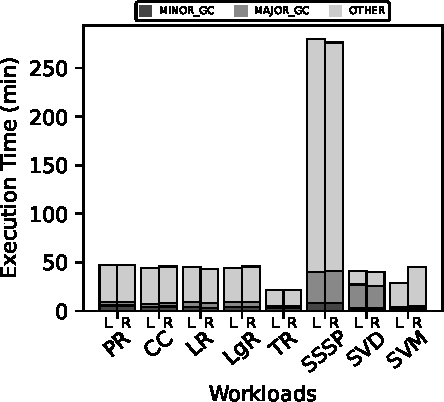
\includegraphics[width=\linewidth]{figures/bench_spark.pdf}\\
\caption{TeraHeap Spark performance. local NVMe device (L) compared to NVMe-oF exported NVMe with SPDK (R).}
\label{fig:bench_spark}
\end{figure}
The two TeraHeap setups local NVMe device (L) and NVMe-oF exported NVMe with
SPDK (R) perform similarly with Spark workloads. We can see that the local setup
outperforms the remote setup in Pagerank(PR), Connected Components(CC), and
Logistic Regression(LgR) making the local setup 0.85\%, 3.55\% and 3.18\% faster
accordingly. The big difference is in the SVM workload where the local setup
outperforms the remote by 37.30\% \textbf{(why????)}. There are also cases where
the remote setup is better. Workloads Linear Regression(LR), Triangle
Counts(TR), Shortest Path(SSSP) and SVDPlusPlus(SVD) report that the remote
setup is 4.76\%, 2.08\%, 1.37\% and 2.76\% quicker accordingly. Spark workloads
read objects from H2 but don't change them  ~\cite{spark,teraheap} so heavy
write operations are missing.

Next, we run TeraHeap with the Giraph workloads. These workloads read objects
from H2 and also change them. Here we expect heavy write operations
~\cite{giraph,teraheap} that can stress the remote setup. Figure
\ref{fig:bench_giraph} illustrates the performance of TeraHeap with Giraph
workloads for both setups NVMe device (L) and NVMe-oF exported NVMe with SPDK
(R).

\begin{figure}[H]
  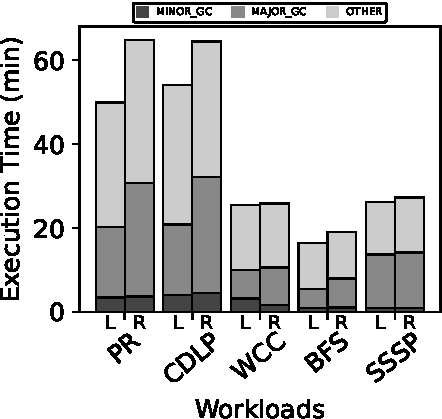
\includegraphics[width=\linewidth]{figures/bench_giraph.pdf}\\
\caption{TeraHeap Giraph performance. local NVMe device (L) compared to NVMe-oF exported NVMe with SPDK (R).}
\label{fig:bench_giraph}
\end{figure}
Here, due to the write operations, the remote setup (R) never manages to exceed the performance of the local setup (L). PageRank (PR), CDLP and BFS workloads are the ones that the remote setup struggles the most here local setup is 22.97\% 16.24\% and 13.07\% quicker accordingly. In the setups mentioned before the remote setup is losing performance due to major GC's taking more time to complete. Following up with WCC and SSSP workloads we can see that the local setup is only 1.54\%	and 3.97\% faster again here major GC's are the reason the remote setup is slower.

\subsection{Workload disk statistics}

 In this section we review the disk statistics of the workload runs. First we
 examine Spark. figures \ref{fig:spark_r} and \ref{fig:spark_w} show reads and
 writes accordingly. First, we can confirm that reads are more than writes due to
 the nature of spark benchmarks. Next focusing on the reads we can see that the
 Gigabytes read for both the local setup (L) and the remote setup (R) are close.
 An exception here is the SVM workload where the remote setup has 8.3$\times$
 more Gigabytes of reads.
 
 Next we examine Giraph. figures \ref{fig:giraph_r} and \ref{fig:giraph_w} show
 reads and writes accordingly. Focusing on the writes we can see that the data
 in Gigabytes for both the local setup (L) and the remote setup (R) are close.
 In the PageRank(PR)	and CDLP workloads where the local setup (L) has the
 best performance compared to the remote setup (R) (figure
 \ref{fig:bench_giraph} 22.97\% and 16.24\% faster) we can see more reads
 (figure \ref{fig:giraph_r}) for the remote setup due to more major GC's.

\begin{figure}[H]
  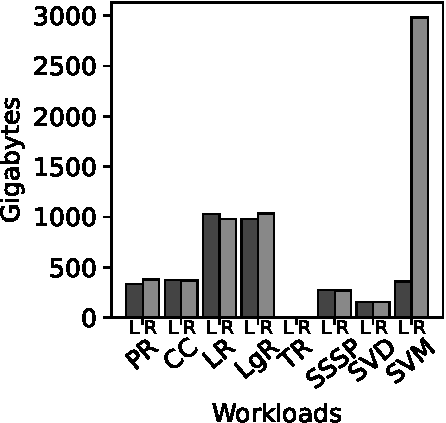
\includegraphics[width=\linewidth]{figures/spark_r.pdf}\\
\caption{TeraHeap Spark workloads reads (GB). local NVMe device (L) compared to NVMe-oF exported NVMe with SPDK (R).}
\label{fig:spark_r}
\end{figure}
\begin{figure}[H]
  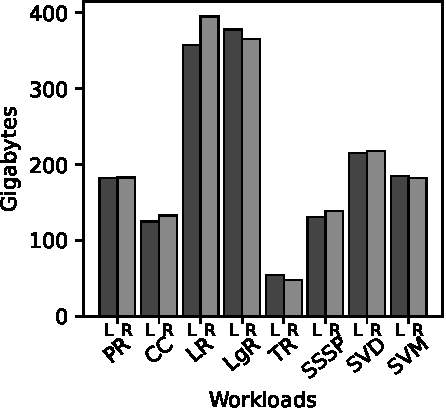
\includegraphics[width=\linewidth]{figures/spark_w.pdf}\\
\caption{TeraHeap Spark workloads writes (GB). local NVMe device (L) compared to NVMe-oF exported NVMe with SPDK (R).}
\label{fig:spark_w}
\end{figure}
\vspace{10em}
\begin{figure}[H]
  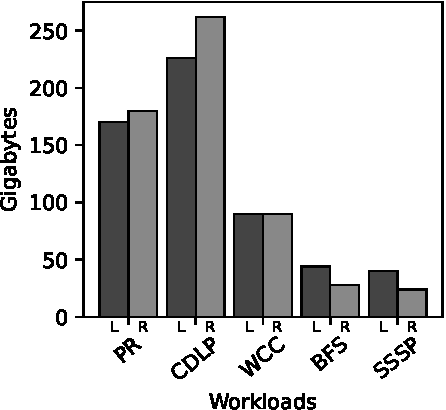
\includegraphics[width=\linewidth]{figures/giraph_r.pdf}\\
\caption{TeraHeap Giraph workloads reads (GB). local NVMe device (L) compared to NVMe-oF exported NVMe with SPDK (R).}
\label{fig:giraph_r}
\end{figure}

\begin{figure}[H]
  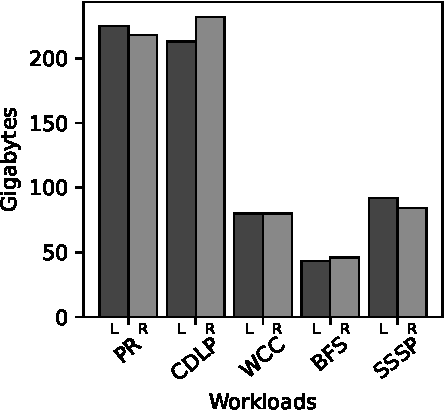
\includegraphics[width=\linewidth]{figures/giraph_w.pdf}\\
\caption{TeraHeap Giraph workloads writes (GB). local NVMe device (L) compared to NVMe-oF exported NVMe with SPDK (R).}
\label{fig:giraph_w}
\end{figure}
